\documentclass{article}
\usepackage[utf8]{inputenc}

\usepackage[backend=bibtex]{biblatex}
\addbibresource{dmu-gnn.bib}
% \usepackage{indentfirst}
\usepackage{hyperref}
\usepackage[a4paper, total={6in, 10in}]{geometry}
\usepackage{amsmath}
\usepackage{graphicx, wrapfig}
\usepackage[utf8]{inputenc} % allow utf-8 input
\usepackage[T1]{fontenc}    % use 8-bit T1 fonts
\usepackage{hyperref}       % hyperlinks
\usepackage{url}            % simple URL typesetting
\usepackage{booktabs}       % professional-quality tables
\usepackage{amsfonts}       % blackboard math symbols
\usepackage{nicefrac}       % compact symbols for 1/2, etc.
\usepackage{microtype}      % microtypography
\usepackage{xcolor}         % colors
\usepackage{float}
\usepackage{tabularx}
\usepackage{xcolor}
\newcommand{\dan}[1]{{\color{purple}DANNY: #1 \\}}
\newcommand{\jelc}[1]{{\color{orange}JULIAN: #1 \\}}
\newcommand{\dpi}[1]{{\color{blue}DANIEL: #1 \\}}

\setlength{\parindent}{0pt}

\title{% 
    Automated Theorem Proving with Graph Neural Networks}
\author{Daniel Jenson, Julian Cooper and Daniel Huang}
% \date{January 20th, 2023}

\begin{document}

\maketitle

% Requirements: Write a 4-6 page paper describing your research. It should follow the typical conference style with an abstract, introduction, etc. State the problem you are trying to solve, introduce your approach, and review the relevant literature. The experiments should be described in sufficient detail so that someone with a reasonable background in the area could reproduce your results. Show your results and discuss the conclusions that can be drawn. You can use the AAAI, AIAA, NIPS, or IEEE paper templates (the LaTeX version looks better, but Word will be accepted)—or you can use the template of another conference of your choice.


% \vspace{-3em}

\begin{center}
\large\textbf{Abstract} \\
\end{center}
By leveraging recent advances in Graph Neural Networks (GNNs), we were able to exceed the performance of TreeLSTM-based models in the CoqGym dataset. The CoqGym dataset consists of roughly 189 thousand mathematical and software verification proofs that use the Coq automated (ATP) and interactive (ITP) theorem prover. Our best model proves 19.4\% of proofs in the ZFC dataset, which consists of 237 proofs regarding Zermelo–Fraenkel set theory. By comparison, ASTactic, the CoqGym author's model proves 14.8\%. Our model uses a combination of a GNN deep encoder with a modified version of a tactic decoder to generate valid tactics for solving proofs.

\section{Problem Statement}
Theorem proving is a difficult, lengthy process, which has historically been the sole employ of mathematicians. Recent engineering and computer science advances have seen the advent of theorem proving assistants. These are software programs that aid mathematicians in proving statements by providing a formal syntax for composing proofs and a verification process for validating them. \\

\begin{figure}[h]
    \centering
    % Kind of small for coq architecture, not sure if that matters much
    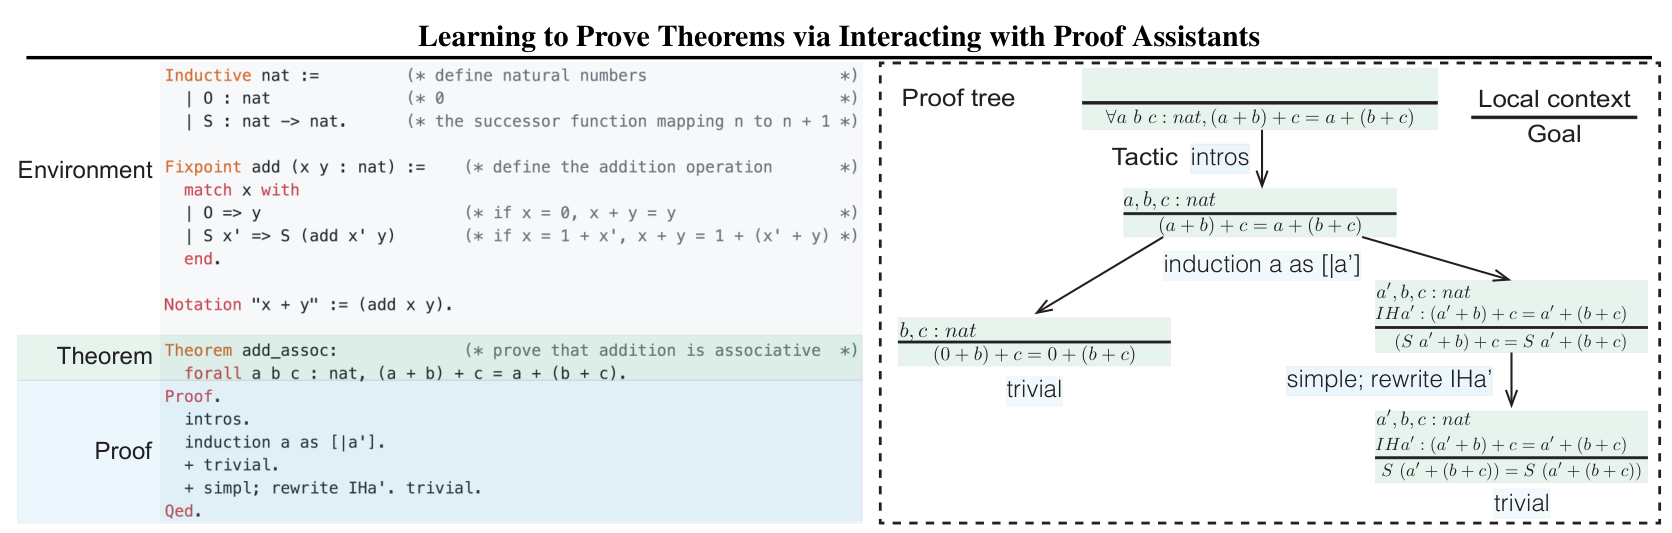
\includegraphics[width=0.9\textwidth]{images/proof_assistant_example.png}
    \caption{Automated Proof Assistant: an example of the induction tactic \cite{coqgym}}
    \label{fig:atp}
\end{figure}

More recently, some of these software programs have begun to provide automated theorem proving (ATP) components, which are capable of automatically selecting tactics and proving simpler sub-goals. Since 2019, these ATP modules have been further augmented with neural networks, creating a new class of ATPs called Neural Theorem Provers (NTPs). NTPs are often structured as an encoder-decoder, which consists of an encoder that embeds goals in a latent space and a decoder that uses these representations to produce a distribution over valid tactics or proof techniques. In this project, we extend one of these NTP frameworks. \\

In this framework we start with a goal (statement to prove) and our agent analyzes existing data (solved proof steps) to develop a model that predicts the next best action, which is the application of a proof tactic, e.g. mathematical induction. This action is then submitted to the environment, which applies the tactic to our goal and returns \texttt{SUCCESS} if solved, or \texttt{UNSOLVED} along with any subgoals that remain to be solved. This interaction progresses the proof one step. The resulting subgoals, along with the context (relevant axioms and proven premises), form our new state. This information is fed into the encoder, which produces new embeddings that the tactic decoder uses to generate the next tactic. This repeats until all subgoals are empty and the proof is complete, or the process terminates because a maximum number of tactics have been applied or it has reached a maximum time limit.

Since our agent's understanding of the problematically best tactic to submit at each step is imperfect, there is model uncertainty. Moreover, the state space is exponentially large with a branching factor much larger than the game of Go \cite{alphago}. The state space consists of MDPs at two levels. At the outer level, the state space consists of proof trees, where each action applies a tactic to create subgoals and generate a new proof tree. At the inner level, the state space consists of tactic trees, where each action adds a node to the tactic tree until it represents a fully-formed tactic that can be applied. The outer level is explored with depth-first search, while the latter uses beam search in conjunction with an attention mechanism.

% Further, while our observations (subgoals) do give us trustworthy information about what is left to prove, these do not necessarily constitute a complete state since our context often will not include everything needed to complete the proof at that step. This is what makes the problem partially observed as well as iterative.

% \begin{wrapfigure}{r}{7.5cm}
%     \centering
%     % Kind of small for coq architecture, not sure if that matters much
%     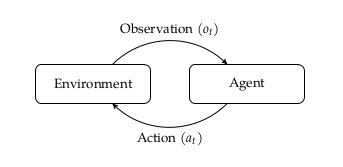
\includegraphics[width=0.5\textwidth]{images/rl-framework.png}
%     \caption{Decision Making Framework \cite{dmu}}
%     \label{fig:rl}
% \end{wrapfigure}
% % \vspace{-3em}
   

\section{Algorithm \& Methodology}
The NTP for our project is composed of two parts: (1) a graph neural network (GNN) encoder and (2) the reinforcement learning agent, which includes a tactic decoder (detailed below). The encoder and decoder are trained with teacher forcing using human proofs. At test time, the reinforcement learning agent uses the output of the model and applies estimated high value tactics to the current goal. It limits the number of tactic applications to 300 and the run-time limit to 10 minutes and is rewarded only when the proof goal and all of its subgoals are proved. \\

There are two principle baselines from existing literature: CoqGym \cite{coqgym} and HOList \cite{hol} CoqGym is based on the Coq theorem proving language and HOList is based on the HOL Light theorem prover. Both implement similar environments for generating states given submitted tactics, but they differ substantively in (a) their representation of goal and premise statements and (b) their encoder-decoder models. Both use abstract syntax trees (ASTs) as their root data type, but Coq uses higher level expressions in the AST. On the other hand, HOList uses a lower-level representation but modifies these ASTs using subexpression sharing, leaf sharing, and random edges in their graph representations. \\

The original Coq NTP paper uses TreeLSTMs to represent the hidden state for terms, while HOList's best model uses a 12-hop GNN. We used CoqGym instead of HOList because the ASTs represented at each proof step capture higher level logic than HOList without requiring significant modifications. Furthermore, until recently, the HOList dataset was not available, and a large portion of the original source code remains unreleased. \\

Another key difference between these models is the scope of tactic generation. HOList limits the number of applicable tactics to 41, while CoqGym's ASTactic can generate a practically infinite number of tactics. In doing so, the HOList GNN can learn to predict which tactics are best where those 41 tactics are viable. However, it inherently limits the flexibility of tactic application. On the other hand, CoqGym's ASTactic can generate any number of tactics. However, these tactics are constructed iteratively, expanding a partial tree until it becomes a valid tactic. This process is slow and expensive. The model also has to learn a much more complicated mapping from current (proof) state to valid tactic.

   \begin{figure}[H]
        \centering
        % Kind of small for coq architecture, not sure if that matters much
        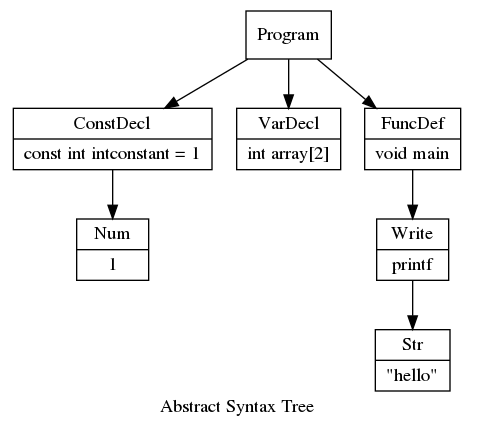
\includegraphics[width=0.5\textwidth]{images/coq-ast.png}
        \caption{Coq's Abstract Syntax Tree (AST) \cite{coqgym}}
        \label{fig:coq_ast}
    \end{figure}

    
\subsection{Extensions to the encoder and agent}
The following details algorithm modifications we made to the term encoder and reinforcement learning agent.

% GNN deep encoder: GraphSage & GAT, mean & max
% rich attention: more layers, layernorm, prelu
% int embedding: more expressive node features
% Training dataset size
% post-pooling Linear layer - suggest we don't mention, not interesting

\begin{enumerate}
    \item \textbf{Graph neural network deep encoder}: The CoqGym paper implemented a TreeLSTM term encoder. We want to improve upon this with a more expressive Graph Neural Network, taking inspiration from the encoder design proposed in Google's HOList paper. Our implementation used two graph convolution layers (2-hop) with ReLU activation and dropout. We experiment with two design choices: (a) GraphSage \cite{graphsage} vs. Graph Attention (GAT) \cite{gat}, and (b) global mean vs. max pooling. GraphSage and GAT differ in how they pass and aggregate messages in the convolution layer. GraphSage assumes messages from neighboring nodes should be equally weighted in importance, whereas GAT allows these weights to vary using an attention mechanism. Global mean and max pooling are two different methods for taking node embeddings we get from convolution layers and generating a single graph embedding. For our problem, the node embeddings each represent individual nodes of a given term AST (single component of the representation of a premise statement, e.g. $\in$ operator), and so pooling across these gives us an embedding for the entire term AST (premise statement, e.g. $a,b,c \in \mathbb{R}$). Mean and max pooling offer different types of information. Mean pool yields an equal weighting on all the nodes, and the embeddings will be expressing what a representative “average node” would look like for the AST while max pooling would highlight individually expressive components of the embedding features over all the nodes. Note, we did not consider global sum pooling since our ASTs vary wildly in size and so some form of normalization would have been required. Differential Pooling is another mechanism we looked into and believe to be very promising, but had to leave for future research.

    \begin{figure}[H]
        \centering
        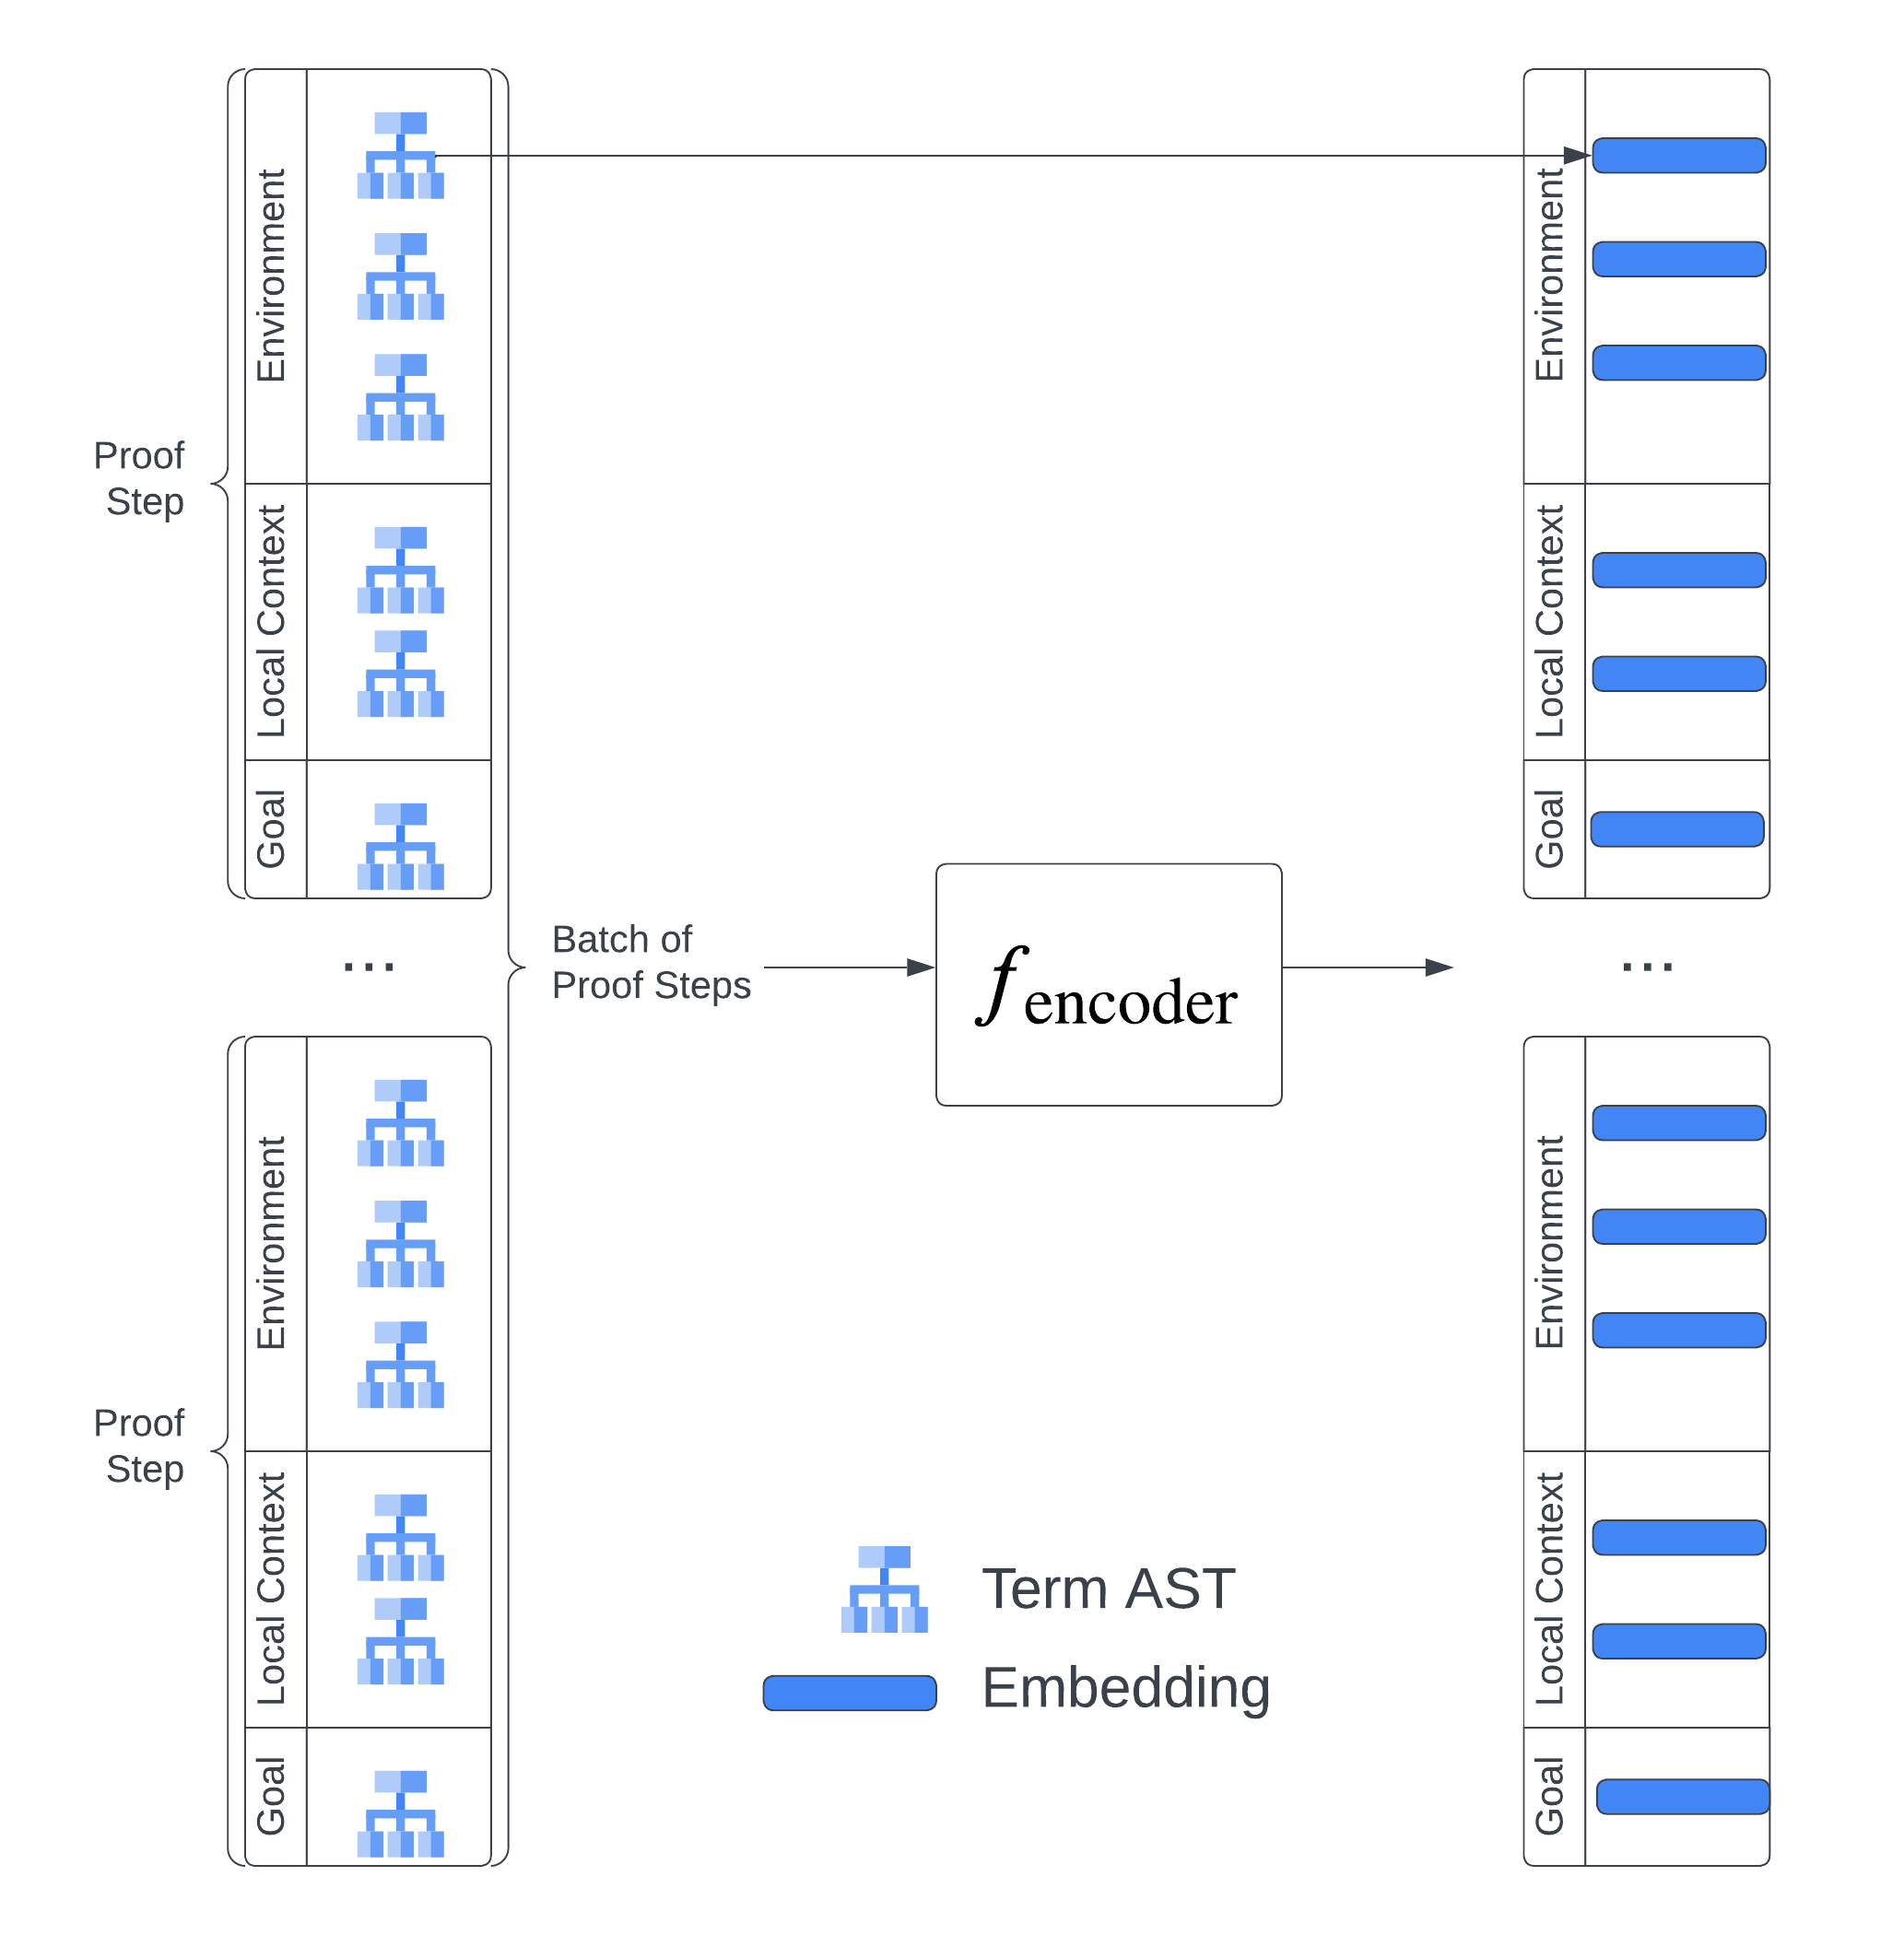
\includegraphics[width=0.7\textwidth]{images/Encoder.png}
        \caption{GNN deep encoder input and output}
        \label{fig:encoder}
    \end{figure}
    
    % \begin{figure}[H]
    %     \centering
    %     % Kind of small for coq architecture, not sure if that matters much
    %     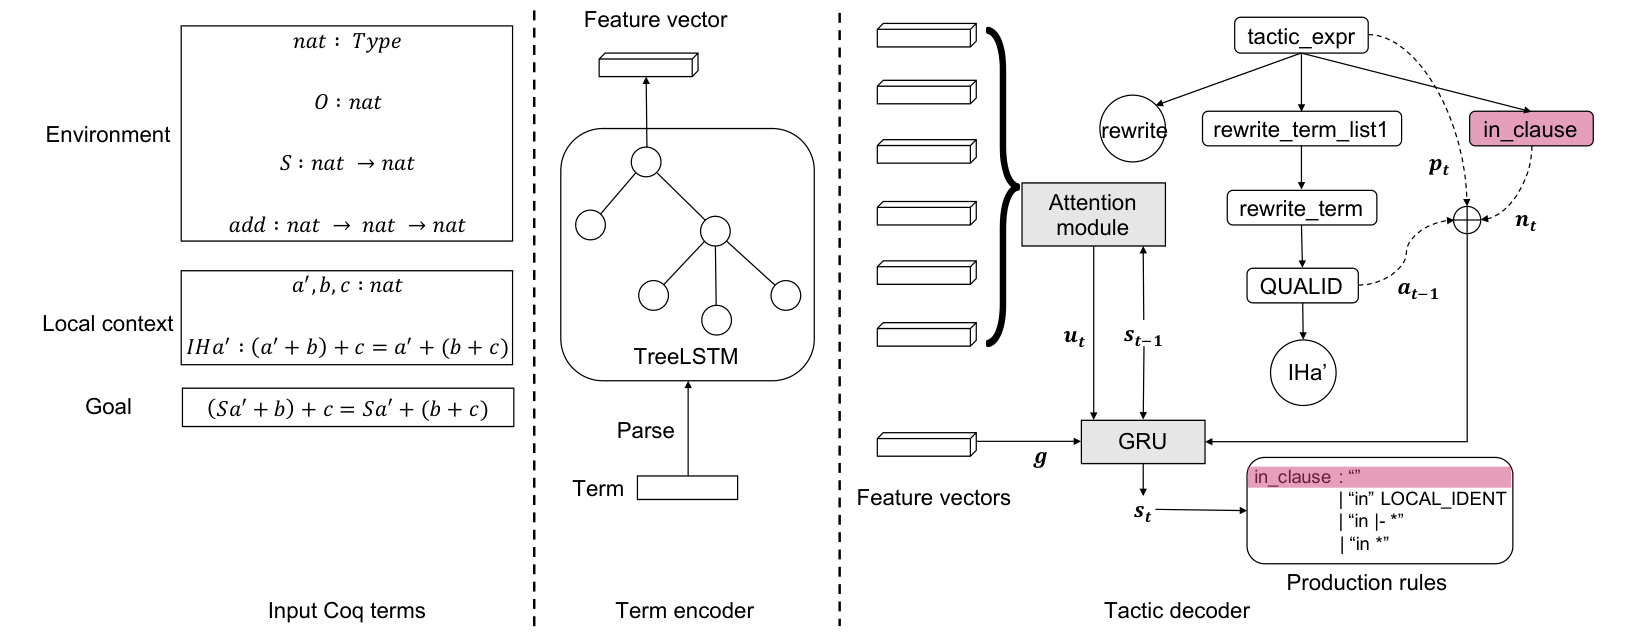
\includegraphics[width=1\textwidth]{images/coqgym.png}
    %     \caption{Coqgym model architecture \cite{coqgym}}
    %     \label{fig:coq_arch}
    % \end{figure}

    \item \textbf{Rich attention for the tactic decoder}: For the tactic decoder, CoqGym used a gated recurrent unit (GRU) with a simple attention mechanism to weight the contribution local context and environment information. The original attention mechanism was a simple two layer feed forward network with a ReLU activation between them. Based on guidance from \cite{prelu} and \cite{layernorm}, we made three changes: (1) we replaced the ReLU activation with a PReLU, (2) we increased the number of layers from two to three, and (3) added layer normalization. In our experiments, this richer attention mechanism had a significant effect on final performance. A PReLU is similar to a ReLU but introduces a learned parameter to allow activation values below zero \cite{prelu}. Increasing the number of layers allows the network to learn more complex functions, and layer normalization largely prevents gradient vanishing and exploding \cite{layernorm}
   
    \begin{figure}[H]
        \centering
        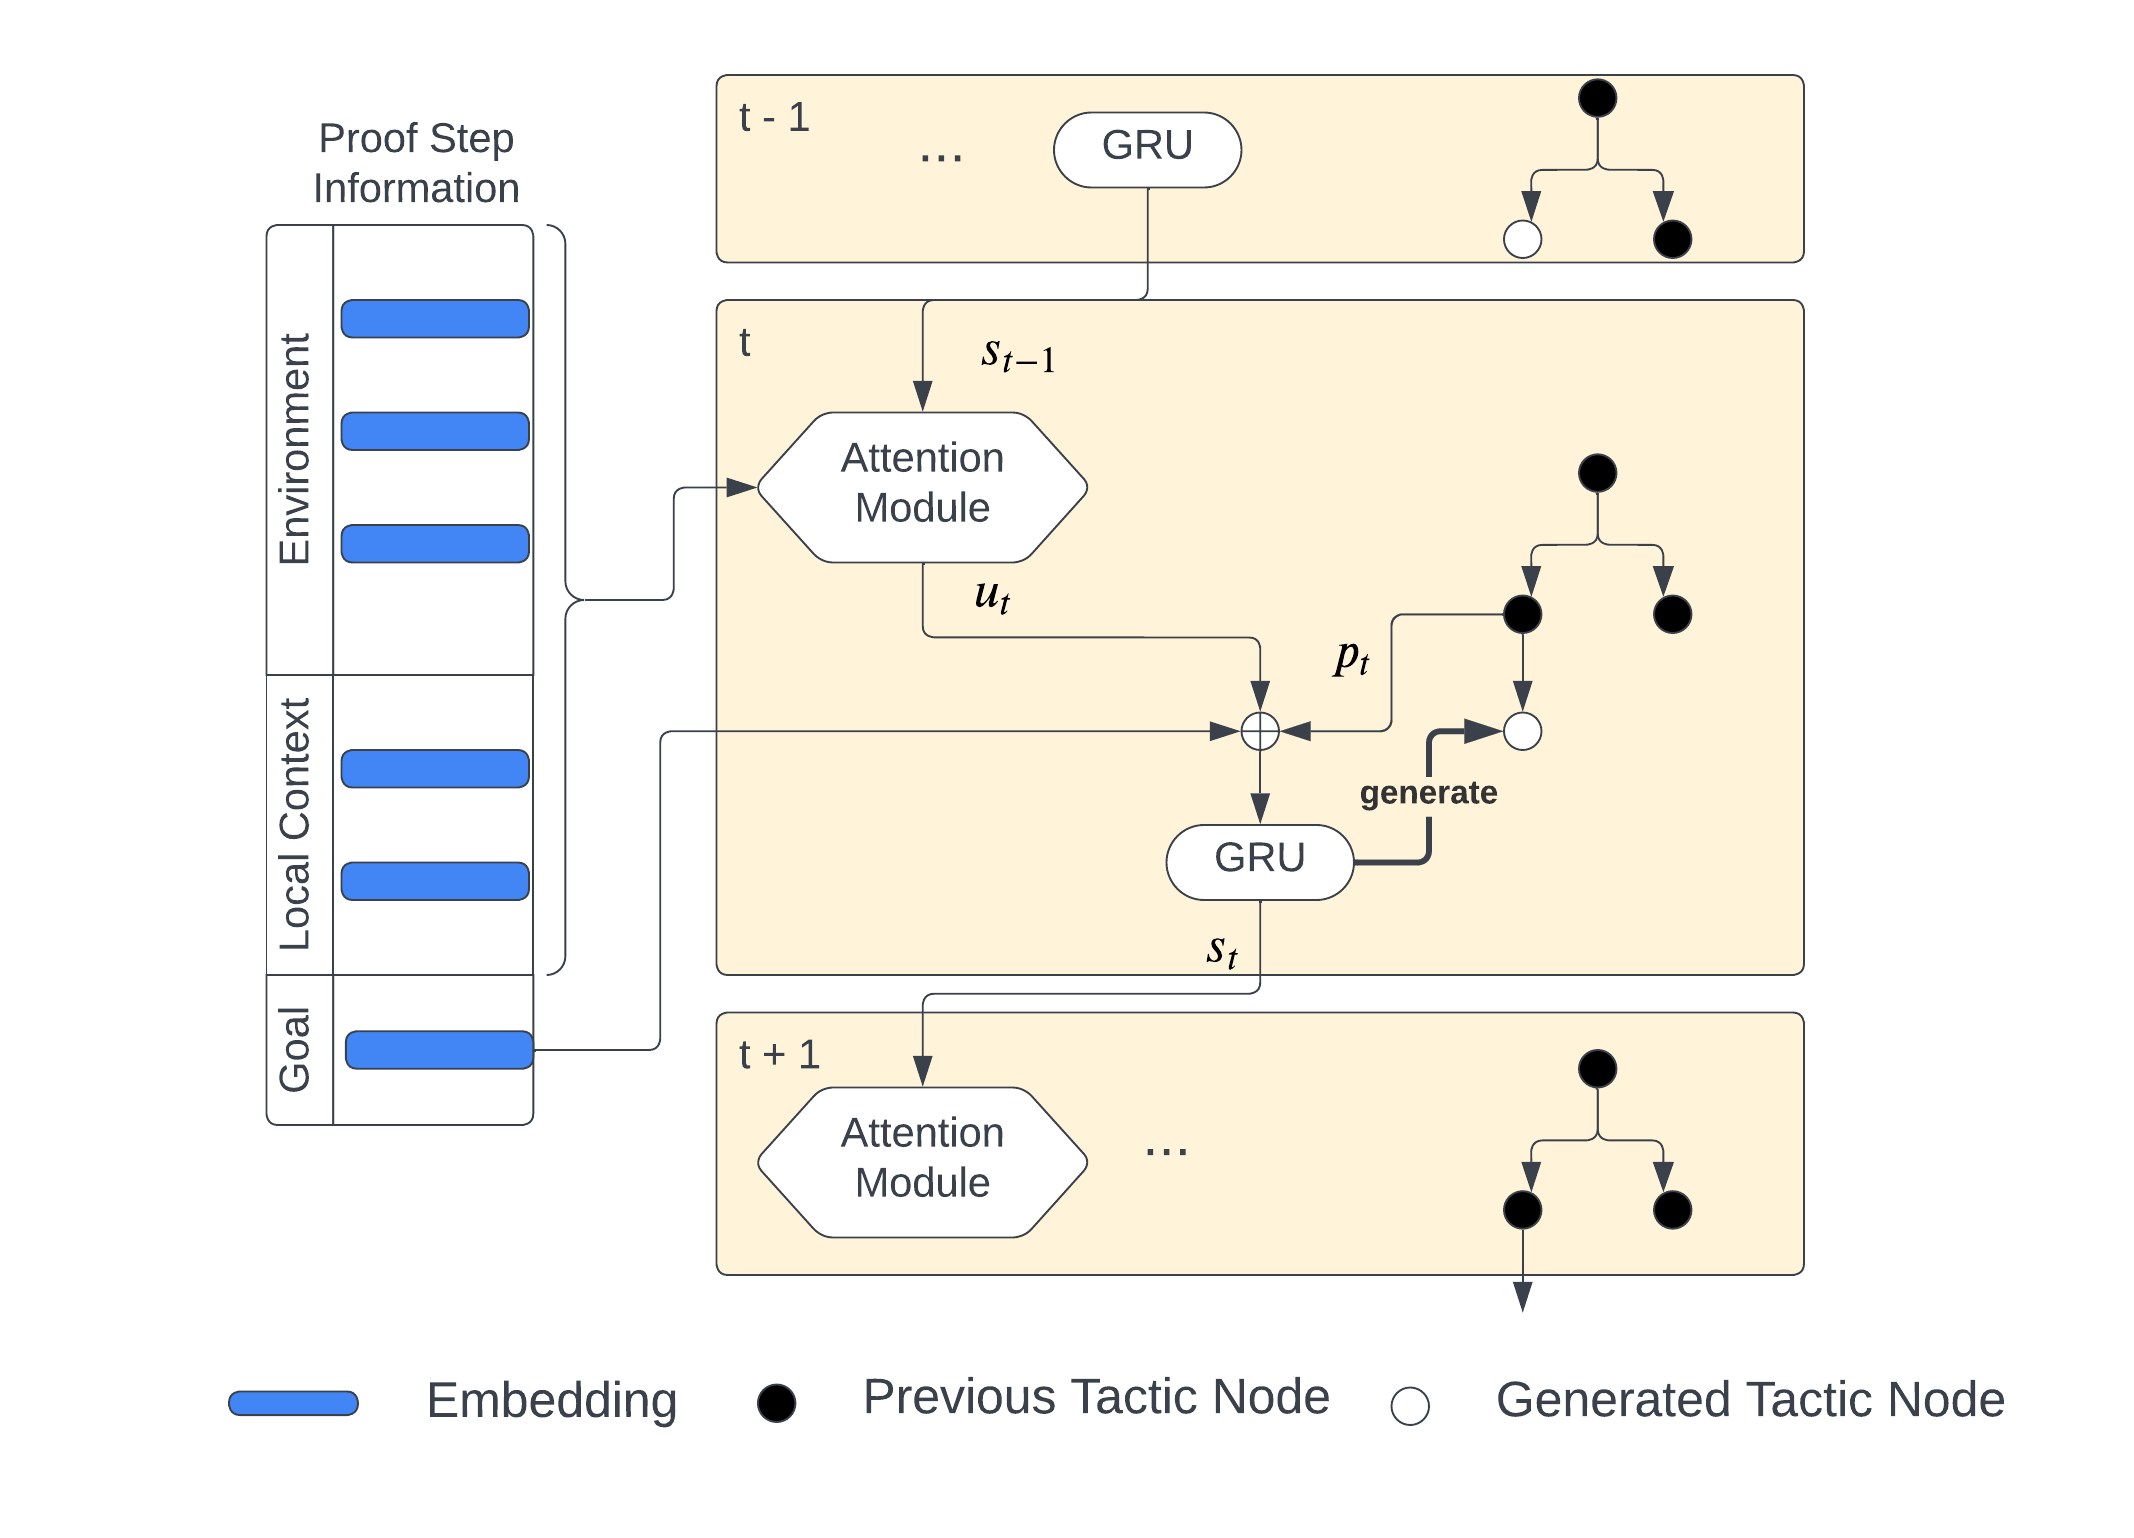
\includegraphics[width=0.7\textwidth]{images/Decoder.png}
        \caption{GNN deep encoder input and output}
        \label{fig:encoder}
    \end{figure}
    
    \item \textbf{Shallow embeddings for node (term) types}: There are multiple ways to initialize node embeddings for our graph neural network encoder: fixed integer, one-hot encoding, integer embedding, centrality-based approaches (e.g. degree, clique reference), or random-walk-based approaches (e.g. DeepWalk, HOPE) \cite{emb}. We decided to make use of GraphGym's integer feature encoder \cite{graphgym} which picks semi-orthogonal directions in $n$-dimensional space for each of our $m>n$ input nodes. As we train the model, these feature vectors are shifted such that similar nodes become closer in the embedding space. This allows our model to transfer learning between embeddings in a localized region of the embedding space and improves the model's capacity to generalize over these features. With sufficient training data, this decreases the memory footprint relative to one-hot encoding, and improves the representation of features in a more compact subspace. 
\end{enumerate}

\textbf{Size of our training set}: Deep neural networks are very data hungry and typically require very large datasets to perform well. CoqGym extracts roughly 189 thousand proof steps to in a teacher-forcing fashion when constructing tactics. Extracting the baseline proof steps using the original ASTactic proof steps requires roughly four CPU hours multiprocessed across 12 cores. However, our GNN model requires a richer representation in order to generate embeddings. Accordingly, we had to extract node features as well as edge indices with the proof steps so that we could construct a graph for every term in every proof step. This increased the data extraction time from approximately 8 hours to nearly 2.5 days. This figure also reflects a number of optimizations (detailed below) that we had to implement. Our original basic extension required nearly 5 days to extract all the data in a format PyGeometric could use. There are some proofs and proof projects that are significant outliers, which stalls extraction for a very long time as all intermediate graphs are constructed and serialized. Given this, we trained models on various size training datasets to understand the effect of the dataset size on performance in the test set.   


\subsection{Extensions to the Coqgym software pipeline}
While our principle focus was on encoder, decoder, and agent extensions, we realized early on that a significant amount of development would be dedicated to improving the development cycle and overcoming inefficiencies in CoqGym's base implementation. In addition to the aforementioned modeling improvements, we also made the following improvements to the underlying platform:

% Reproducing original training/testing pipeline
% proof steps, tweaked dataloader,  Batch of batches
% Retool encoding-decoding pipeline for GNN edits
% (put rough associated times with all of these)
% Multiprocess evaluation (& timing)

\begin{enumerate}
    % \item \textbf{Reproduced Coqgym training and testing pipelines locally}: The installation process is very complex, requiring the installation of OCaml and a variety of packages, the compilation of a custom version of the Coq theorem proving software, the extraction of proofs from the Coq language to ASTs that can be manipulated in Python, and the compilation of other external theorem proving agents called ``hammers.'' This process requires approximately 12 hours of computation (with more time debugging potential errors) and 55 GB of storage. We also had to submit several fixes and improvements to this process, since the existing code was broken or underspecificied (e.g. missing PyTorch version). This process needed to be reproduced multiple times on 4 personal devices and 3 servers to provide flexibility in evaluating multiple models.

    \item \textbf{Proof step data augmentation and batching}: PyGeometric graphs require node features and edge indices for construction. Accordingly, we had to extract that data and serialize it in a format that PyGeometric could use. This dramatically increased the size of the serialized proof steps. Furthermore, this required that we modify the dataloader so that it could use an object that carried elements we required to encode term ASTs as graph embeddings as well as all the additional information the tactic decoder required to utilize this embedding in building tactics. A particularly tricky part of this implementation involved retooling the batching process. Each proof step might contain hundreds of environment and local context terms, as well as a goal term. Each of these terms is represented as an tree graph (AST) in PyGeometric. So, a batch, which consists of several proof steps, often contains thousands of graphs. Ensuring that the environment, local context, and goal embeddings are properly extracted and attributed to the correct proof step was a subtle enterprise, especially since we needed to combine these encoded terms with the metadata that was part of the original batch.

    \item \textbf{Parallelized proof extraction and evaluation}: The scripts provided for proof extraction and evaluation processes each proof in series. This causes the extraction process on the entire dataset to take approximately 12 hours (over 5 days for extracting all PyGeometric graph object information) and much longer for evaluation (on the order of days or weeks). These processes are trivially parallelizable, so we implemented a multiprocessing script to process each proof in parallel. With further optimizations to their iteration process, the data extraction ended up taking roughly 2.5 days including all PyGeometric graph objects. However for evaluation, the optimizations did not bring down the evaluation time as the process is significantly limited by the serial process of searching the proof tree. This is why we limit our testing for this project to the subset of proofs in the ZFC project. At 237 proofs, we felt the ZFC project represented a sufficiently large dataset to compare the performance of models employing different techniques and inform the evolution of our experiemnts.
        
    
\end{enumerate}
\section{Results \& Discussion}
For evaluating the effectiveness our various model extensions, we selected an example proof library (known as ZFC) with 237 human-written proofs as our baseline. These proofs are taken from Zermelo–Fraenkel set theory which is a well-studied branch of mathematics. In future research we would like to expand this test set to include all proof libraries used to generate CoqGym's published benchmarks, but due to limited time and computational resources, we narrowed the scope of our testing pipeline for this project. \\

%  that we assume has a nearly complete set of human proofs to provide effective teacher-forcing

We run experiments testing a variety of extensions on ~65\% of the training dataset, including: (a) GraphSage vs. GAT term encoder, (b) global mean vs. max pooling,  (c) one-hot vs. integer feature encoding, and (d) rich vs. simple attention in the decoder.
\begin{table}[h]
\begin{tabular}{ccccccc}
\hline
Ref & Conv. Type & Pooling & Attention & Embedding & Accuracy (\%) & Correct (/237) \\ \hline
1   & GraphSage  & max     & rich      & integer   & \textbf{17.7\% }       & 42     \\
2   & GraphSage  & mean    & rich      & integer   & 13.1\%        & 31             \\
3   & GAT        & max     & rich      & integer   & 11.4\%        & 27             \\
4   & GAT        & mean    & rich      & integer   & \textbf{15.2\%}        & 36      \\
5   & GAT        & mean    & rich      & one-hot   & 13.1\%          & 31             \\ 
6   & GAT        & mean    & simple   & integer   & 10.6\%        & 25             \\ \hline
\end{tabular}
\caption{Accuracy results for encoder-decoder model variants using ZFC proof library.}
\label{t1}
\end{table}

From our experimental results on the partial dataset, we learned a lot. First, by comparing models 4, 5 and 6, we find that both our rich attention and integer feature encoder modifications were valuable improvements. Second, it is not clear whether global mean or max pooling is more appropriate for this problem since they perform differently for each of the different convolution layer types. And third, while GraphSage appeared to perform better than GAT, then delta was small enough that both appeared in our two best models. \\

For each of the results in the Table \ref{t1}, we show the results from our best performing epoch (up to 10). CoqGym used 5 epochs for its ASTactic model and they commented that their performance did not improve meaningfully after epochs 3-4. While we also observed a similar trend, we did find substantial improvements in epochs 5-10 for some of our models, likely because the GNN-based models had far more trainable parameters (see figure \ref{fig:epochs}).

\begin{figure}[H]
    \centering
    % Kind of small for coq architecture, not sure if that matters much
    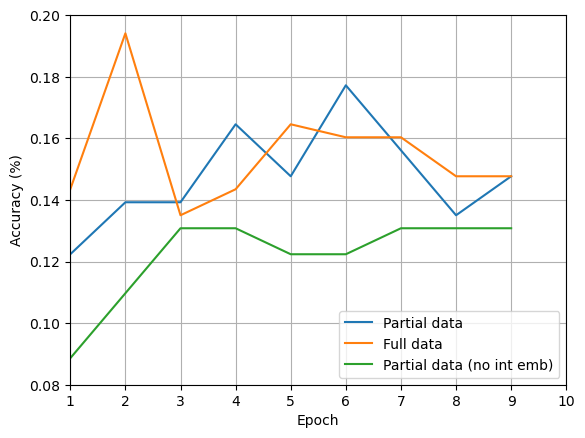
\includegraphics[width=0.7\textwidth]{images/int-emb-GraphSage-max.png}
    \caption{Performance for three example models over epochs 1-9}
    \label{fig:epochs}
\end{figure}

Having experimented with different modifications, we picked the two best performing models (highlighted in Table \ref{t1}) to train on the full dataset and benchmark against CoqGym's ASTactic results for the ZFC proof library. We present these results in Table \ref{t2}.
\begin{table}[h]
\begin{tabular}{lcccccc}
\hline
Ref       & Conv. Type & Pooling & Attention & Embedding & Accuracy (\%) & Correct (/237) \\ \hline
ASTactic  & n/a        & n/a     & n/a       & n/a       & 14.8\%        & 35             \\
Model \#1 & GraphSage  & max     & rich      & integer   & \textbf{19.4\% }       & 46     \\
Model \#4 & GAT        & mean    & rich      & integer   & 17.3\%        & 41             \\ \hline
\end{tabular}
\caption{Benchmark accuracy results for our two best performing models trained on the full dataset}
\label{t2}
\end{table}

\section{Conclusion}
In this project, we have found that GNNs are a viable and performant alternative to TreeLSTMs in generating proof tactics and proofs. Our best model, a max-pooled, integer-feature embedded, rich attention GraphSage neural network achieved 19.4\% on the ZFC test set, while ASTactic achieved 14.8\%. While this is a modest improvement, we view this as a promising start, as we have a number of enhancements we wish to test that we believe will further increase the expressive power of the generated embeddings.

\section{Next Steps}
Given that nearly half of our development time was devoted to software enhancements rather than model experimentation and testing, we plan to continue working on this next quarter. In particular, we plan on experimenting with ID-GNNs, which are provably the most expressive GNNs, as well as Differential Pooling, which creates a more intelligent graph embeddings from node embeddings using hierarchical clustering. We also plan on using more ``hops,'' in our network, as HOList saw improvements up to 12 hops and we only used 2. Lastly, we believe we can improve the agent further by experimenting with different tactic search mechanisms, perhaps using Monte Carlo Tree Search in lieu of depth-first search. We also plan on experimenting with another theorem proving program, Isabelle, and it's publicly available Archive of Formal Proofs (AFP), which is notably easier to manipulate than CoqGym's proofs and serialized internals.


\newpage
\textit{Contributions: Dan Jenson owned setup of our remote server, multiprocessing and software extensions to the CoqGym pipeline. Julian Cooper owned development of extensions to the term encoder. Daniel Huang owned development of updates to the term decoder and assisted in optimizing data augmentation and extraction. Everyone contributed to brainstorming GNN and RL design choices, testing and evaluation methodology and sense checking results.}

\printbibliography
\end{document}
